\section{Proof Details}
\label{sec:ibhc-proof}

\treerefinement*
\begin{proof}
\TODO{Change the T}

Suppose, first, that $T$ is a refinement of $T'$. Pick any triplet $(\{a,b\},c) \in \Delta(T')$. Then there is a node in $T'$ whose descendants include $a,b$ but not $c$. By the definition of refinement, $T$ contains a node with the same descendants. Hence the constraint $(\{a,b\},c)$ holds for $T$ as well.

Conversely, say $\Delta(T') \subseteq \Delta(T)$. Pick any cluster $S'$ of $T'$; it consists of the descendants of some node in $T'$. Consider the set of all triplet constraints consisting of two nodes of $S'$ and one node outside $S'$. Since these constraints also hold for $T$, it follows that the lowest common ancestor of $S'$ in $T$ must have exactly $S'$ as its set of descendants. Thus $S'$ is also a cluster of $T$.
\end{proof}

\irreducible*
\begin{proof}
To prove irreducibility, we show that there is a non-zero probability
of moving from state $T$ to $T'$, both of which satisfy $C$. We
accomplish this by first defining a \emph{canonical tree} $T_C$ given a triplet 
set $C$ and showing that we can reach $T_C$ from $T$ using  
constrained-SPR moves. We then show that for every constrained-SPR move,
there exists an equivalent reverse move that undoes it with non-zero
probability.
This proves that that from $T_C$ we can reach $T'$, 
creating a path from $T$ to $T_C$ to $T'$.

A binary tree $T$ can be entirely defined by the bipartitions
made over the data at each node. 
Let $G_n$ be the Aho graph for node $n$.
For a binary tree that satisfies a set of triplets, 
the split over the data at each node $n$ must 
be a bipartition of the connected components of $G_n$.
We define a particular node to be in \emph{canonical form}
if either a) it is a leaf, or b) the bipartition over $G_n$
at that node can be written as
$(l, r)$, where $l$ exactly matches a single, particular connected component of
$G_n$, and $r$ is the rest of the connected components. 
The particular component
$l$ is the connected component in $G_n$ with the minimum data index
inside it.
Note that we treat the children of nodes as unordered.
A canonical tree $T_C$ is one such that every node in the tree is
in canonical form.
To convert an arbitrary tree $T$ that satisfies $C$ into $T_C$, we first
convert the root node of $T$ into canonical form
using constrained-SPR moves.

Let $s$ be the root of $T$ and let $l$
be the set of points that ought to be in their own partition according
to $G_s$. In order for
$s$ not to be in canonical form, $l$ must be in a partition with 
data from other connected components in $G_s$, which we will call $o$.
The bipartition if $s$ were in canonical form would be $(l, r)$ and
the current non-canonical bipartition can thus be written as $(l + o, r - o)$.

We first examine $t$, the child of the root that contains $l + o$.
In general, the data from $l$ and the data from $o$ could
be split over the children of $t$, so the partition at $t$
can be written as $(l_1 + o_1, l_2 + o_2)$ where $l = l_1 + l_2$ 
and $o = o_1 + o_2$. This is visualized in the first
tree of \autoref{fig:canonical}.
We first group the data from $l$ into their own ``pure'' subtree
of $t$ as follows.
Let $u$ be the root of the
lowest non-pure subtree of $t$ that has
data from $l$ in both of its children.
There exist two subtrees that are descendants of $u$ 
that contain data from $l$ (one on the left and one on the right).
Those two subtrees
must be pure, and furthermore, they are both free to
move within $u$ via constrained-SPR moves because
they are in different connected components in $G_u$.
Thus, we can perform a constrained-SPR move to merge these
two pure subtrees together into a larger pure subtree.
We can repeat this process for $t$ until all nodes
from $l$ are in their own pure subtree of $t$.
The partition of $t$ can thus be written as
$(l + o_1, o_2)$, since the pure subtree may be several
levels down from $t$. This grouping process is visualized in
\autoref{fig:canonicalgrouping} and the results can be
seen in the second
tree in \autoref{fig:canonical}.

\begin{figure}
    \centering
    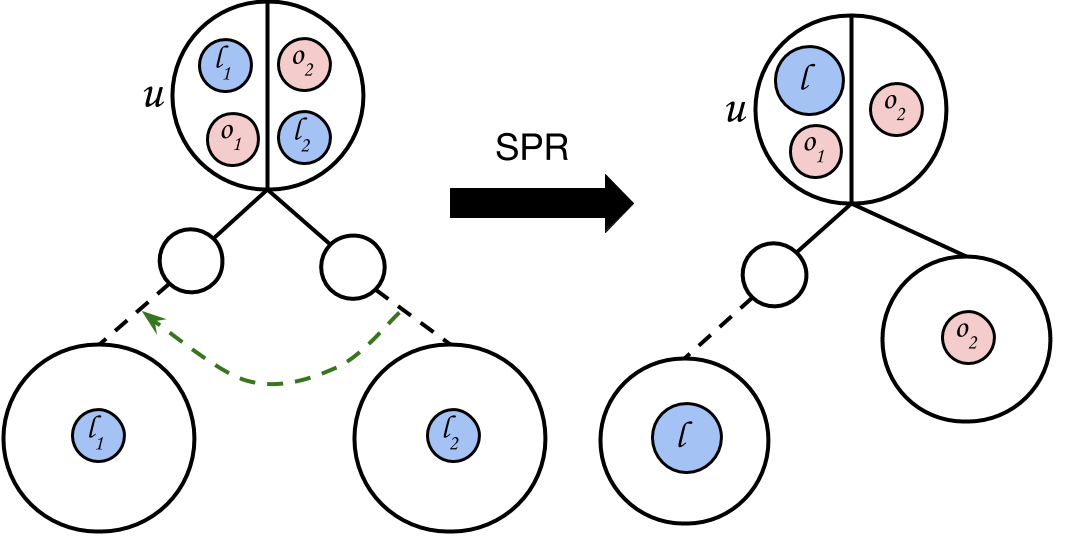
\includegraphics[width=0.5\textwidth]{img/ibhc/CanonicalTreeGrouping}
    \caption{The process of grouping the data in $u$
    that belong to $l$ into their own pure subtree. $u$ is the
    lowest node of $t$ (see \autoref{fig:canonical}) that has data from $l$
    in both of its children.}
    \label{fig:canonicalgrouping}
\end{figure}


We now perform a constrained-SPR move to detach
the pure subtree of $l$ and regraft it to
the edge between $s$ and $t$. This is a permissible
move since $l$ is its own connected component in 
$G_s$. We now have the third tree in \autoref{fig:supcanonical}.
We now perform a final constrained-SPR
move, moving the subtree of $o$ to the opposite
side of $s$, creating the proper canonical partition
of $(l, r)$.
To entirely convert $T$ into $T_C$, we need to recurse
and convert every node in $T$ into canonical form.

\begin{figure*}
    \centering
    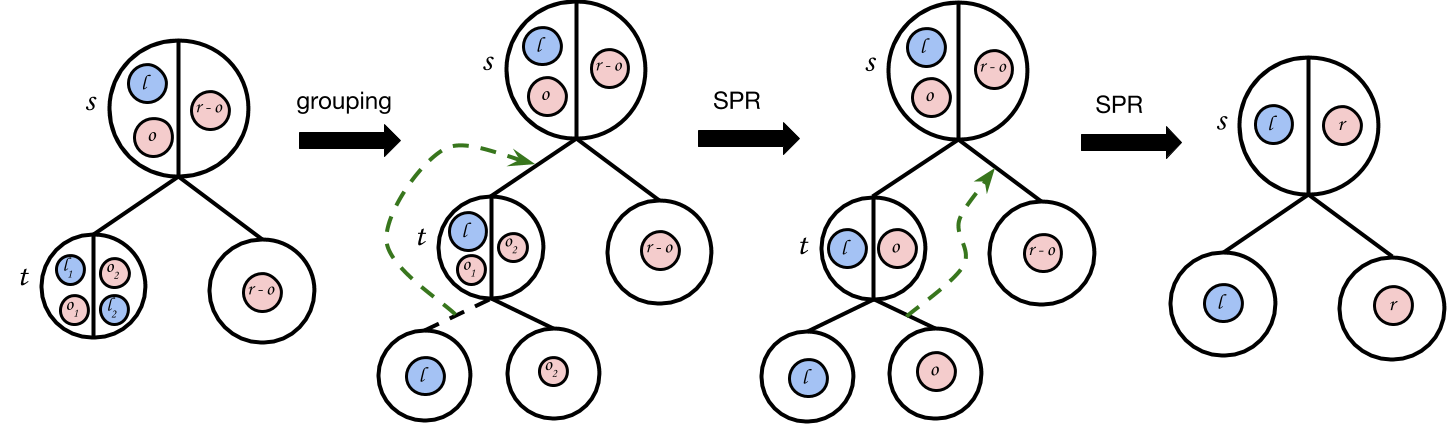
\includegraphics[width=\textwidth]{img/ibhc/CanonicalTree}
    \caption{The process of converting $s$ into canonical form.
    We first group nodes from $l$ into their own pure subtree, then perform
    two constrained-SPR moves to put $s$ into canonical form.}
    \label{fig:supcanonical}
\end{figure*}

Every constrained-SPR move has an associated reverse constrained-SPR move that
performs the opposite transition.
The reverse constrained-SPR move selects the same subtree as the forward one
and prunes it, and just regrafts the subtree to its original location
before the forward move.
We know that this regraft has non-zero probability because the original tree
did not violate constraints.
Thus, since any arbitrary $T$ can be converted into $T_C$ and since each move
has a non-zero probability reverse move,
$T_C$ can be converted into an arbitrary tree $T'$ and we have a non-zero probability
path to convert $T$ into $T'$.

\end{proof}

\section{Additional Results}

\begin{figure*}[h]
    \begin{subfigure}[b]{0.5\textwidth}
        \centering
        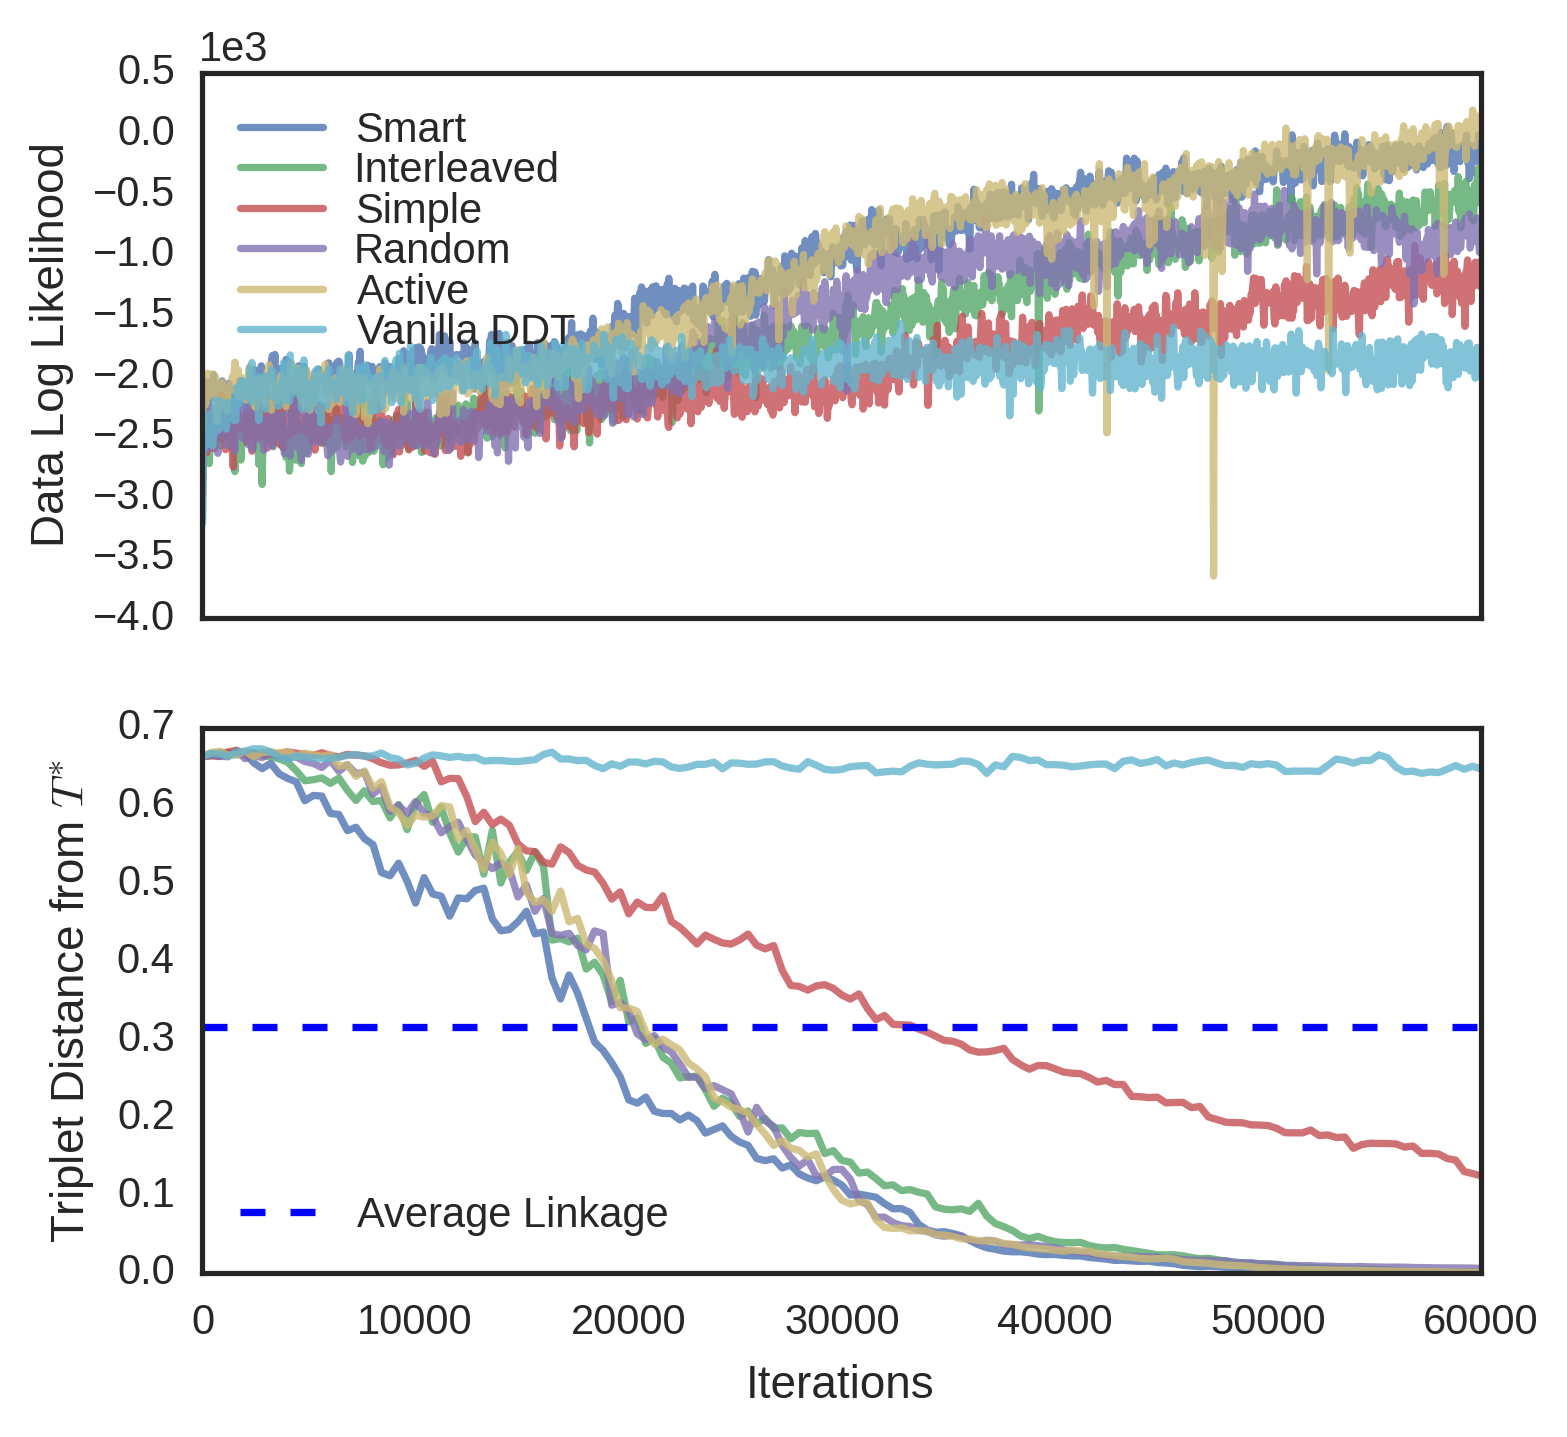
\includegraphics[width=\textwidth]{img/ibhc/Zoo-result.png}
        \caption{Zoo}
        \label{fig:zoo-result}
    \end{subfigure}
    \begin{subfigure}[b]{0.5\textwidth}
        \centering
        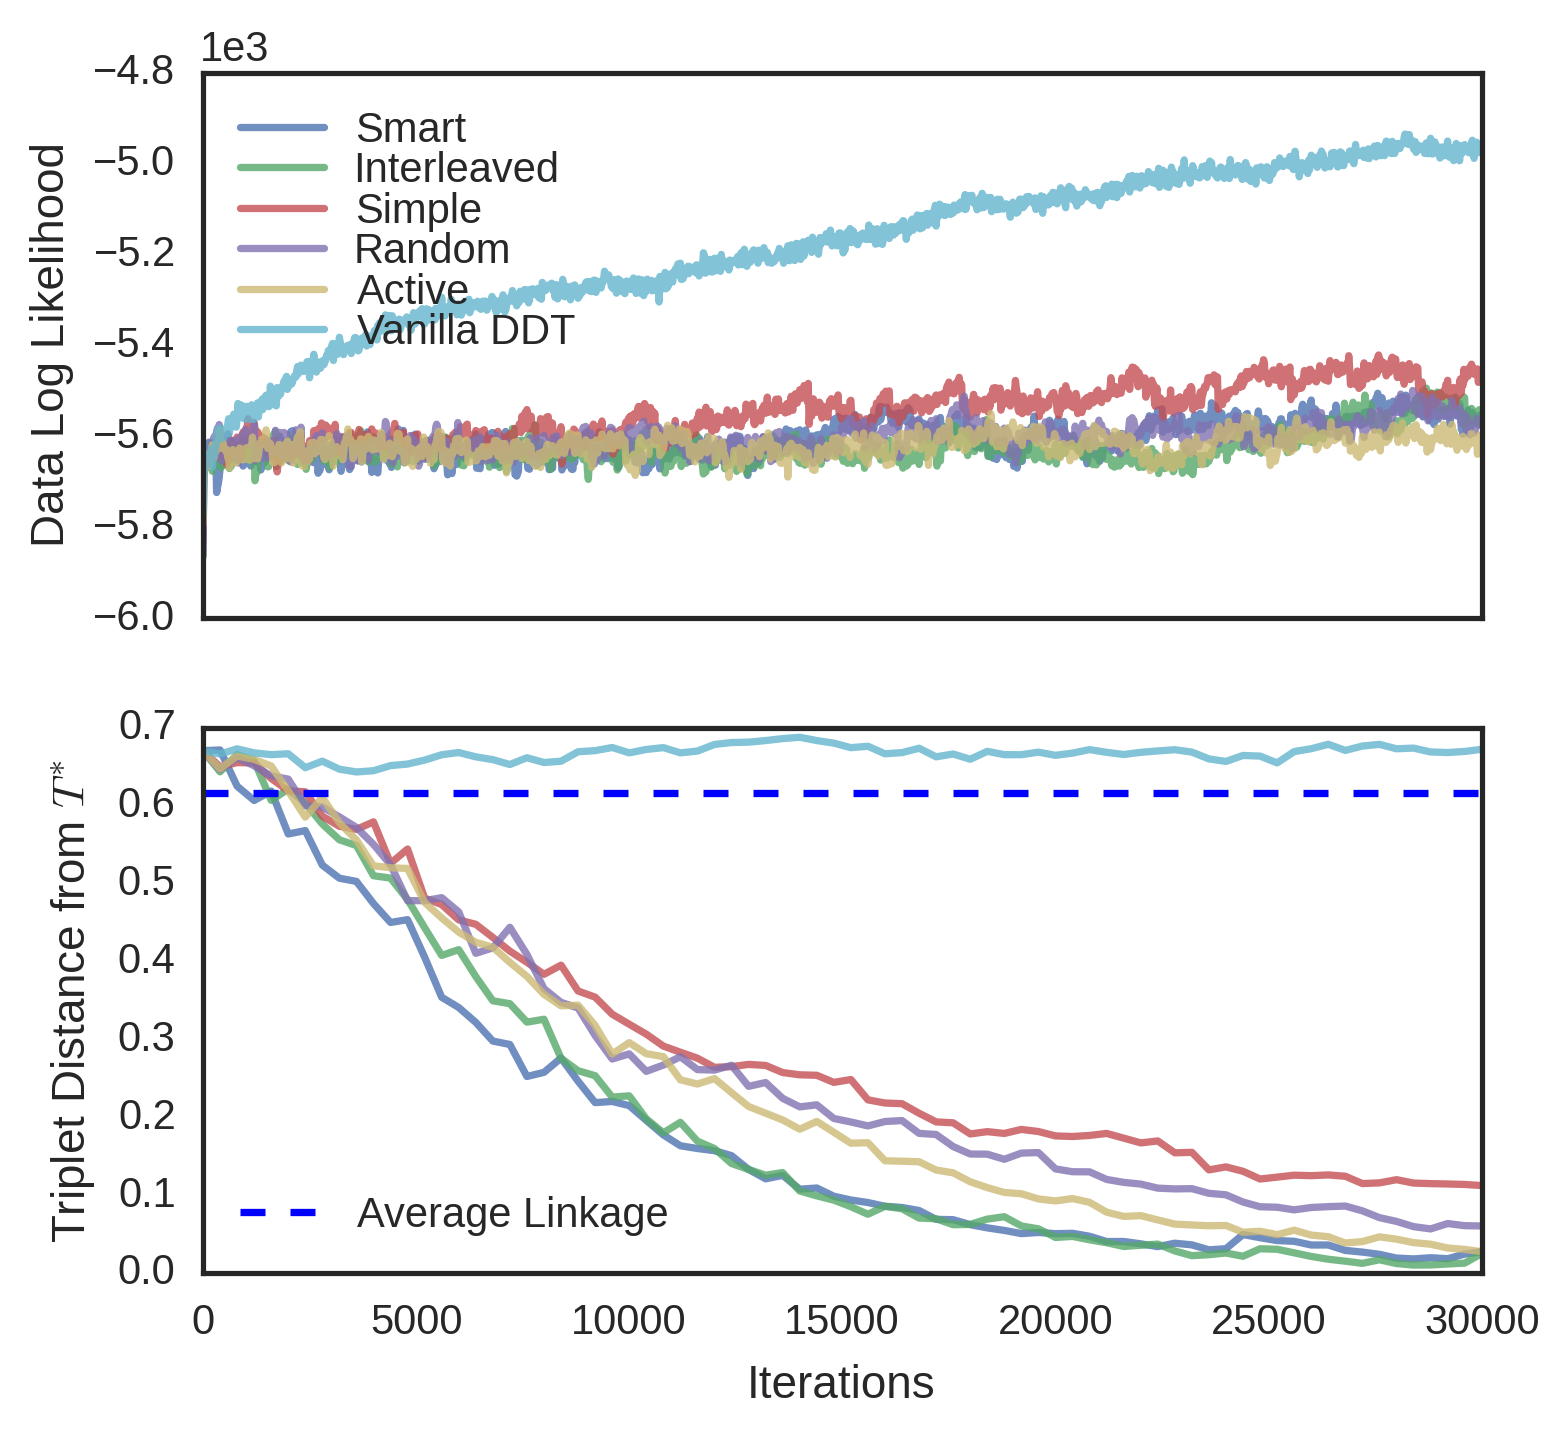
\includegraphics[width=\textwidth]{img/ibhc/20-Newsgroups-result.png}
        \caption{20 Newsgroups}
        \label{fig:20news-result}
    \end{subfigure}
    \caption{The average of four runs of constrained-SPR samplers
        for the Zoo dataset and the 20 Newsgroups dataset, using 5 different querying schemes.
        A query was made every 100 iterations.}
    \label{fig:main-results2}
\end{figure*}
